\documentclass[floatsintext,man]{apa6}

\usepackage{amssymb,amsmath}
\usepackage{ifxetex,ifluatex}
\usepackage{fixltx2e} % provides \textsubscript
\ifnum 0\ifxetex 1\fi\ifluatex 1\fi=0 % if pdftex
  \usepackage[T1]{fontenc}
  \usepackage[utf8]{inputenc}
\else % if luatex or xelatex
  \ifxetex
    \usepackage{mathspec}
    \usepackage{xltxtra,xunicode}
  \else
    \usepackage{fontspec}
  \fi
  \defaultfontfeatures{Mapping=tex-text,Scale=MatchLowercase}
  \newcommand{\euro}{€}
\fi
% use upquote if available, for straight quotes in verbatim environments
\IfFileExists{upquote.sty}{\usepackage{upquote}}{}
% use microtype if available
\IfFileExists{microtype.sty}{\usepackage{microtype}}{}

% Table formatting
\usepackage{longtable, booktabs}
\usepackage{lscape}
% \usepackage[counterclockwise]{rotating}   % Landscape page setup for large tables
\usepackage{multirow}		% Table styling
\usepackage{tabularx}		% Control Column width
\usepackage[flushleft]{threeparttable}	% Allows for three part tables with a specified notes section
\usepackage{threeparttablex}            % Lets threeparttable work with longtable

% Create new environments so endfloat can handle them
% \newenvironment{ltable}
%   {\begin{landscape}\begin{center}\begin{threeparttable}}
%   {\end{threeparttable}\end{center}\end{landscape}}

\newenvironment{lltable}
  {\begin{landscape}\begin{center}\begin{ThreePartTable}}
  {\end{ThreePartTable}\end{center}\end{landscape}}




% The following enables adjusting longtable caption width to table width
% Solution found at http://golatex.de/longtable-mit-caption-so-breit-wie-die-tabelle-t15767.html
\makeatletter
\newcommand\LastLTentrywidth{1em}
\newlength\longtablewidth
\setlength{\longtablewidth}{1in}
\newcommand\getlongtablewidth{%
 \begingroup
  \ifcsname LT@\roman{LT@tables}\endcsname
  \global\longtablewidth=0pt
  \renewcommand\LT@entry[2]{\global\advance\longtablewidth by ##2\relax\gdef\LastLTentrywidth{##2}}%
  \@nameuse{LT@\roman{LT@tables}}%
  \fi
\endgroup}


  \usepackage{graphicx}
  \makeatletter
  \def\maxwidth{\ifdim\Gin@nat@width>\linewidth\linewidth\else\Gin@nat@width\fi}
  \def\maxheight{\ifdim\Gin@nat@height>\textheight\textheight\else\Gin@nat@height\fi}
  \makeatother
  % Scale images if necessary, so that they will not overflow the page
  % margins by default, and it is still possible to overwrite the defaults
  % using explicit options in \includegraphics[width, height, ...]{}
  \setkeys{Gin}{width=\maxwidth,height=\maxheight,keepaspectratio}
\ifxetex
  \usepackage[setpagesize=false, % page size defined by xetex
              unicode=false, % unicode breaks when used with xetex
              xetex]{hyperref}
\else
  \usepackage[unicode=true]{hyperref}
\fi
\hypersetup{breaklinks=true,
            pdfauthor={},
            pdftitle={Measuring Lay Theories of Parenting and Child Development},
            colorlinks=true,
            citecolor=blue,
            urlcolor=blue,
            linkcolor=black,
            pdfborder={0 0 0}}
\urlstyle{same}  % don't use monospace font for urls

\setlength{\parindent}{0pt}
%\setlength{\parskip}{0pt plus 0pt minus 0pt}

\setlength{\emergencystretch}{3em}  % prevent overfull lines


% Manuscript styling
\captionsetup{font=singlespacing,justification=justified}
\usepackage{csquotes}
\usepackage{upgreek}



\usepackage{tikz} % Variable definition to generate author note

% fix for \tightlist problem in pandoc 1.14
\providecommand{\tightlist}{%
  \setlength{\itemsep}{0pt}\setlength{\parskip}{0pt}}

% Essential manuscript parts
  \title{Measuring Lay Theories of Parenting and Child Development}

  \shorttitle{Measuring Parenting Theories}


  \author{Emily Hembacher\textsuperscript{1}~\& Michael C. Frank\textsuperscript{1}}

  % \def\affdep{{"", ""}}%
  % \def\affcity{{"", ""}}%

  \affiliation{
    \vspace{0.5cm}
          \textsuperscript{1} Stanford University  }

  \authornote{
    Add complete departmental affiliations for each author here. Each new
    line herein must be indented, like this line. Enter author note here.
    
    Correspondence concerning this article should be addressed to Michael C.
    Frank, 450 Serra Mall, Stanford, CA 94301. E-mail:
    \href{mailto:mcfrank@stanford.edu}{\nolinkurl{mcfrank@stanford.edu}}
  }


  \abstract{Enter abstract here. Each new line herein must be indented, like this
line.}
  \keywords{keywords \\

    \indent Word count: X
  }





\usepackage{amsthm}
\newtheorem{theorem}{Theorem}[section]
\newtheorem{lemma}{Lemma}[section]
\theoremstyle{definition}
\newtheorem{definition}{Definition}[section]
\newtheorem{corollary}{Corollary}[section]
\newtheorem{proposition}{Proposition}[section]
\theoremstyle{definition}
\newtheorem{example}{Example}[section]
\theoremstyle{definition}
\newtheorem{exercise}{Exercise}[section]
\theoremstyle{remark}
\newtheorem*{remark}{Remark}
\newtheorem*{solution}{Solution}
\begin{document}

\maketitle

\setcounter{secnumdepth}{0}



\section{Introduction}\label{introduction}

There is a longstanding interest in individual differences in parenting
behaviors, how they intersect with culture, socioeconomic status, child
outcomes

Parents and caregivers play critical role in forging the environment
that children develop in. As such, developmentalists have long been
interested in variability in parenting behaviors and its effects on the
developing child.

The array of individual parenting behaviors we observe may emerge from
distinct lay parenting theories, or dimensions of belief on which people
differ

The array of individual parenting behaviors we observe may emerge in
part from distinct lay theories that parents hold about parenting and
child development. For example, a parent who believes that children's
later success will be determined by learning opportunities in infancy
may spend more time speaking and reading to their infant. These theories
may or may not be explicit; even implicit theories that are not
articulated have been shown to determine behaviors in other domains
(find examples?).

Previous research on parenting has often focused on a) parenting
behaviors, e.g., Baumrind's scale authoritative/authoritarian, or b)
knowledge about child development. Theories about what is BEST for
children may be a related but distinct construct.

In order to test whether lay theories organize parents' thinking about
parenting and child development, we sought to create a survey measure of
parenting attitudes.

A lay theory framework has been used to conceptualize other types of
beliefs (summarize some examples)

Can we identify distinct theories that parents differ in their
endorsement of? From a methodological perspective, this would mean that
people respond to a set of propositions in a way that suggests one or
more distinct lay theories are driving responses to individual ideas In
the present work, we identify 3 dimensions of parenting attitudes on
which parents differ. We do this by generating a large set of
propositions regarding parenting and child development, and eliciting
adults' agreement ratings for those propositions. We used dimension
reduction techniques to identify 3 factors contributing to people's
responses. We examined the propositions that loaded strongly onto each
factor to better understand the underlying lay theories/attitudes that
might map onto the factors. Through an iterative process, we proceeded
by retaining items that loaded strongly onto one of the factors, and
removing those that did not. As recommended by (), we generated more
propositions that were related to those propositions that were retained.
We completed 9 iterations, after which we retained 24 propositions, with
8 in each subscale.

After finalizing the structure of the survey, we sought to confirm the
external validity of the measure. We did this by asking whether parents'
attitudes as measured by the survey would predict their self-reported
parenting behaviors or their uptake of new parenting information. We
also asked whether demographic variables are associated with differences
in parenting attitudes, or whether different groups (i.e., a general
sample vs.~parents with memberships at a children's museum) would differ
in their attitudes. In the following sections, we provide more detail
about the process of generating and validating the questionnaire.

There are two reasons to focus on parents' lay theories. First, parents'
lay theories might be an important explanatory factor for many of the
behaviors parents engage in with their child. For example, a parent who
believes that building a strong emotional bond with their baby is one of
the most important goals of parenting might have more physical contact
with their child than a parent who does not hold this theory. Secondly,
parents' lay theories may moderate the uptake of new information about
parenting. It is well-established that people more easily encode new
information that is consistent with an existing schema or mental model
they hold (Bransford \& Johnson, 1972). In addition, previous research
has found that interventions on public health beliefs are more
successful when they take into account people's existing belief
structures in the domain (Kumar et al., 2015).

There is some evidence supporting the notion that parents' behaviors are
mediated by implicit lay theories about child development, which vary by
SES and across cultures. For example, cross-cultural studies have found
profound differences in how parents interact with infants. Richman,
Miller, and LeVine (1992) found that mothers in the Gusii community of
Kenya primarily engaged with their children to soothe them when upset,
but did not often speak to them with the goal of engaging or stimulating
them, as did Caucasian parents in the United States. The authors
attribute this behavior to cultural conventions stemming from the belief
that there is no purpose in speaking to infants, as they will not
understand what is being said (LeVine, 2004; Richman et al., 1992).

There are also important differences in how parents within western
cultures interact with their children. Numerous studies have identified
SES disparity in the amount that parents talk to their children, which
in turn predicts children's language and academic outcomes (Hoff, 2003;
Huttenlocher, Vasilyeva, Cymerman, \& Levine, 2002). In an effort to
identify the source of this disparity, Rowe (2008) discovered that
parents' knowledge of child development (as indexed by their scores on
the Knowledge of Infant Development Inventory; KIDI) predicted their
child-directed language, with more knowledgeable parents speaking to
their children more even when controlling for the amount of speech
directed at another adult. Although this study examined parents'
knowledge, and not their lay theories \emph{per se}, it provides
evidence that people's domain knowledge has real consequences for their
interactions with their children.

In the following sections, we describe the process of generating scale
items and initial steps towards validating the scale. To construct the
scale, we followed a structured plan, generating items based on our
review of the literature on parenting attitudes and practices and then
using dimension reduction techniques to identify latent factors (i.e.,
implicit theories) driving people's responses (Clark \& Watson, 1995;
Furr, 2011; Simms, 2008). We then conducted a series of studies aimed at
estimating ecological validity for the scale. Specifically, we asked
whether people's parenting attitudes as assessed by the PAQ varied based
on demographic factors, whether people's attitudes were related to their
self-reported parenting behaviors, and whether attitudes mediated
people's understanding of and memory for new information about parenting
and child development.

\section{Scale Construction}\label{scale-construction}

\begin{figure}
\centering
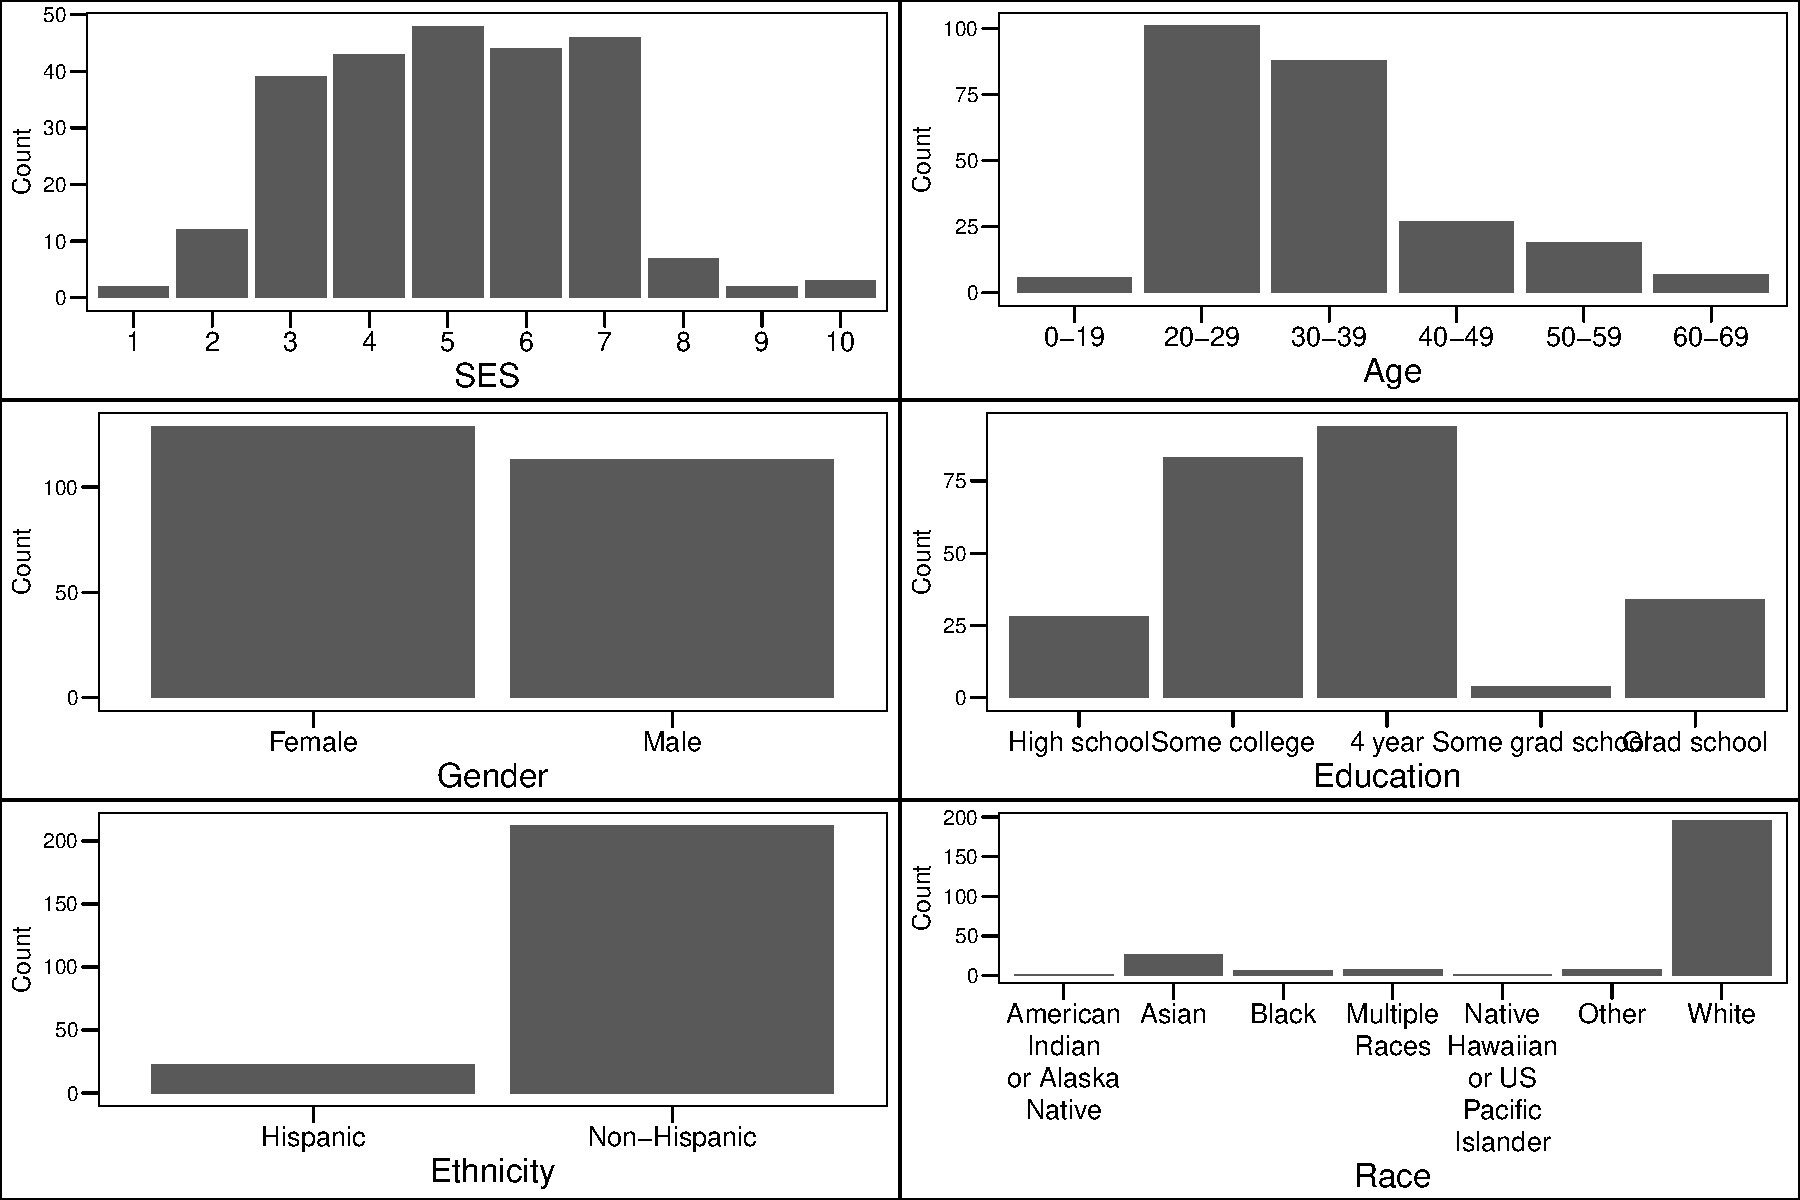
\includegraphics{PAQ_paper_files/figure-latex/normdemo-1.pdf}
\caption{\label{fig:normdemo}Demographic information for participants in the
final norming sample.}
\end{figure}

\begin{figure}
\centering
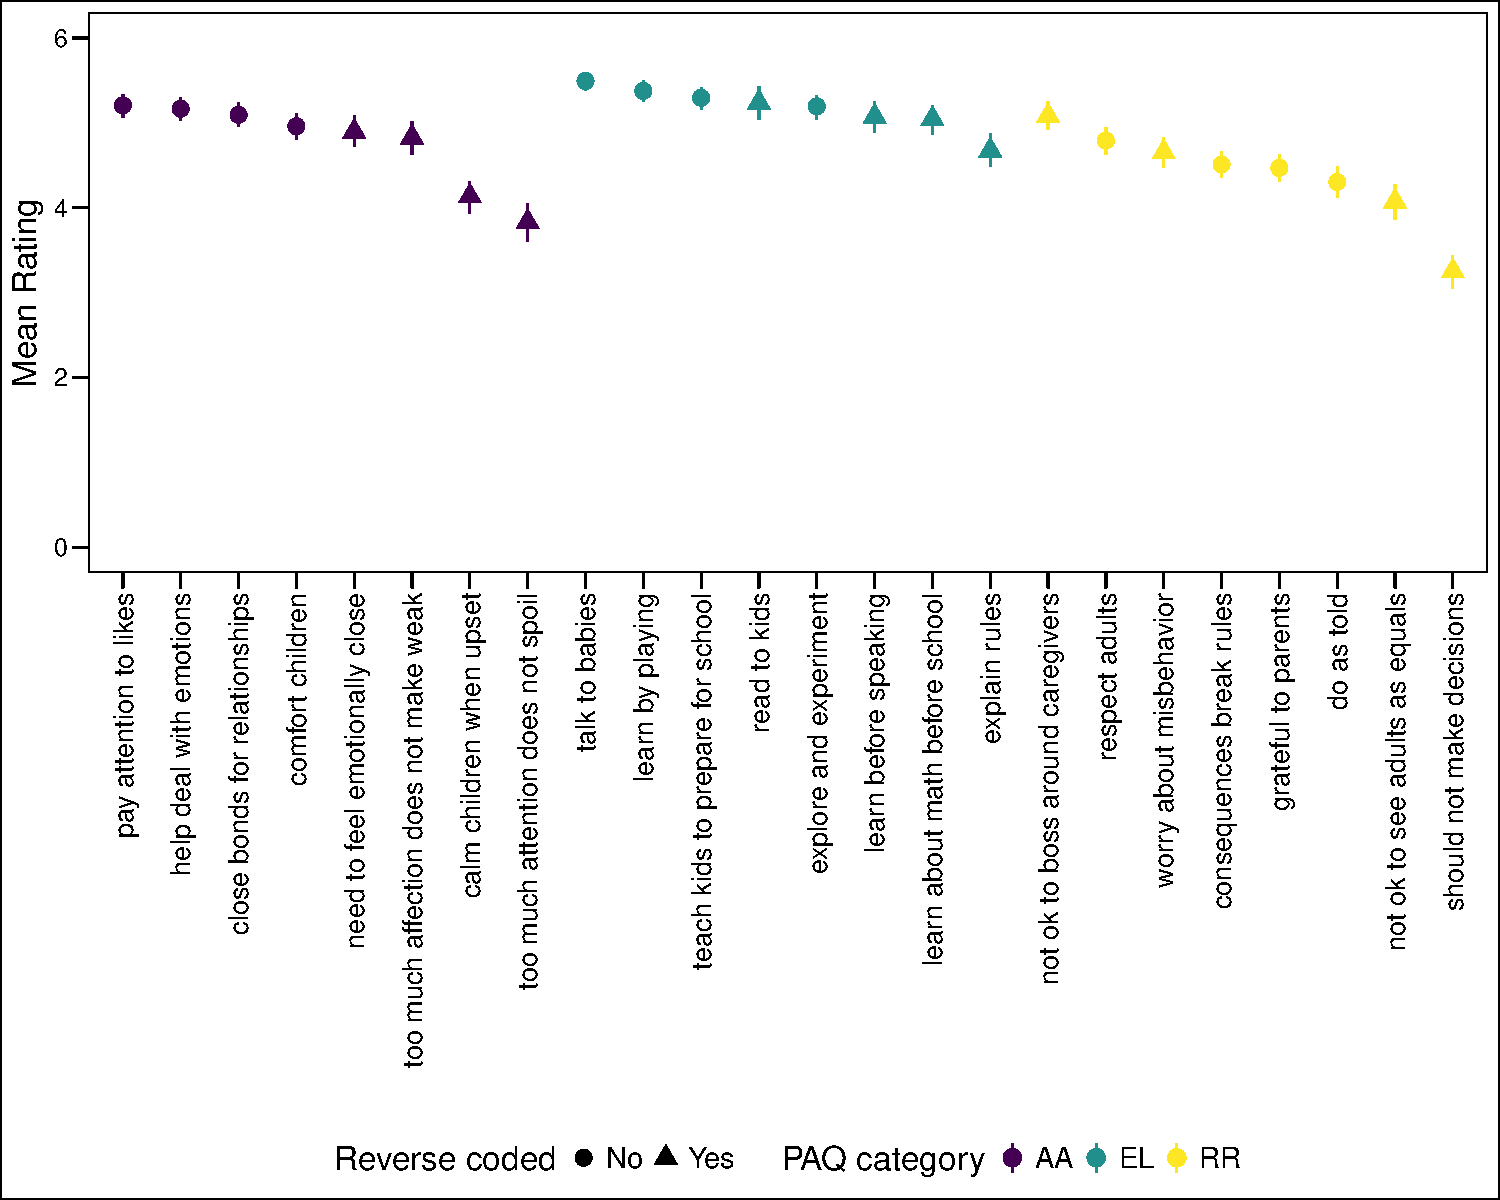
\includegraphics{PAQ_paper_files/figure-latex/sentratings-1.pdf}
\caption{\label{fig:sentratings}Average ratings for individual PAQ items.}
\end{figure}

\begin{table}[!h]

\caption{\label{tab:itemstab}Parenting Attitudes Scale items.}
\centering
\fontsize{9}{11}\selectfont
\begin{tabular}[t]{>{\bfseries}l>{\raggedright\arraybackslash}p{40em}}
\toprule
Category & Item\\
\midrule
AA & Children should be comforted when they are scared or unhappy.\\
 & Its important for parents to help children learn to deal with their emotions.\\
 & Parents should pay attention to what their child likes and dislikes.\\
 & A child who has close bonds with his or her parents will have better relationships later on in life.\\
 & Children who receive too much attention from their parents become spoiled.*\\
\addlinespace
 & Too much affection, such as hugging and kissing, can make a child weak.*\\
 & Children and parents do not need to feel emotionally close as long as children are kept safe.*\\
 & Parents should not try to calm a child who is upset, it is better to let children calm themselves.*\\
EL & It is good to let children explore and experiment.\\
 & Parents can help babies learn language by talking to them.\\
\addlinespace
 & Parents can prepare young children to succeed in school by teaching them things, such as shapes and numbers.\\
 & Babies can learn a lot just by playing.\\
 & It is not helpful to explain the reasons for rules to young children because they wont understand.*\\
 & Children dont need to learn about numbers and math until they go to school.*\\
 & Reading books to children is not helpful if they have not yet learned to speak.*\\
\addlinespace
 & Babies cant learn about the world until they learn to speak.*\\
RR & It is very important that children learn to respect adults, such as parents and teachers.\\
 & It is very important for young children to do as they are told, for example, waiting when they are told to wait.\\
 & Children should be grateful to their parents.\\
 & It is very important that there are consequences when a child breaks a rule, big or small.\\
\addlinespace
 & It is okay if young children boss around their caregivers.*\\
 & It is okay if children see adults as equals rather than viewing them with respect.*\\
 & Young children should be allowed to make their own decisions, like what to play with and when to eat.*\\
 & Parents do not need to worry if their child misbehaves a lot.*\\
\bottomrule
\multicolumn{2}{l}{\textit{Note: }}\\
\multicolumn{2}{l}{*Indicates reverse coded items.}\\
\end{tabular}
\end{table}

\begin{figure}
\centering
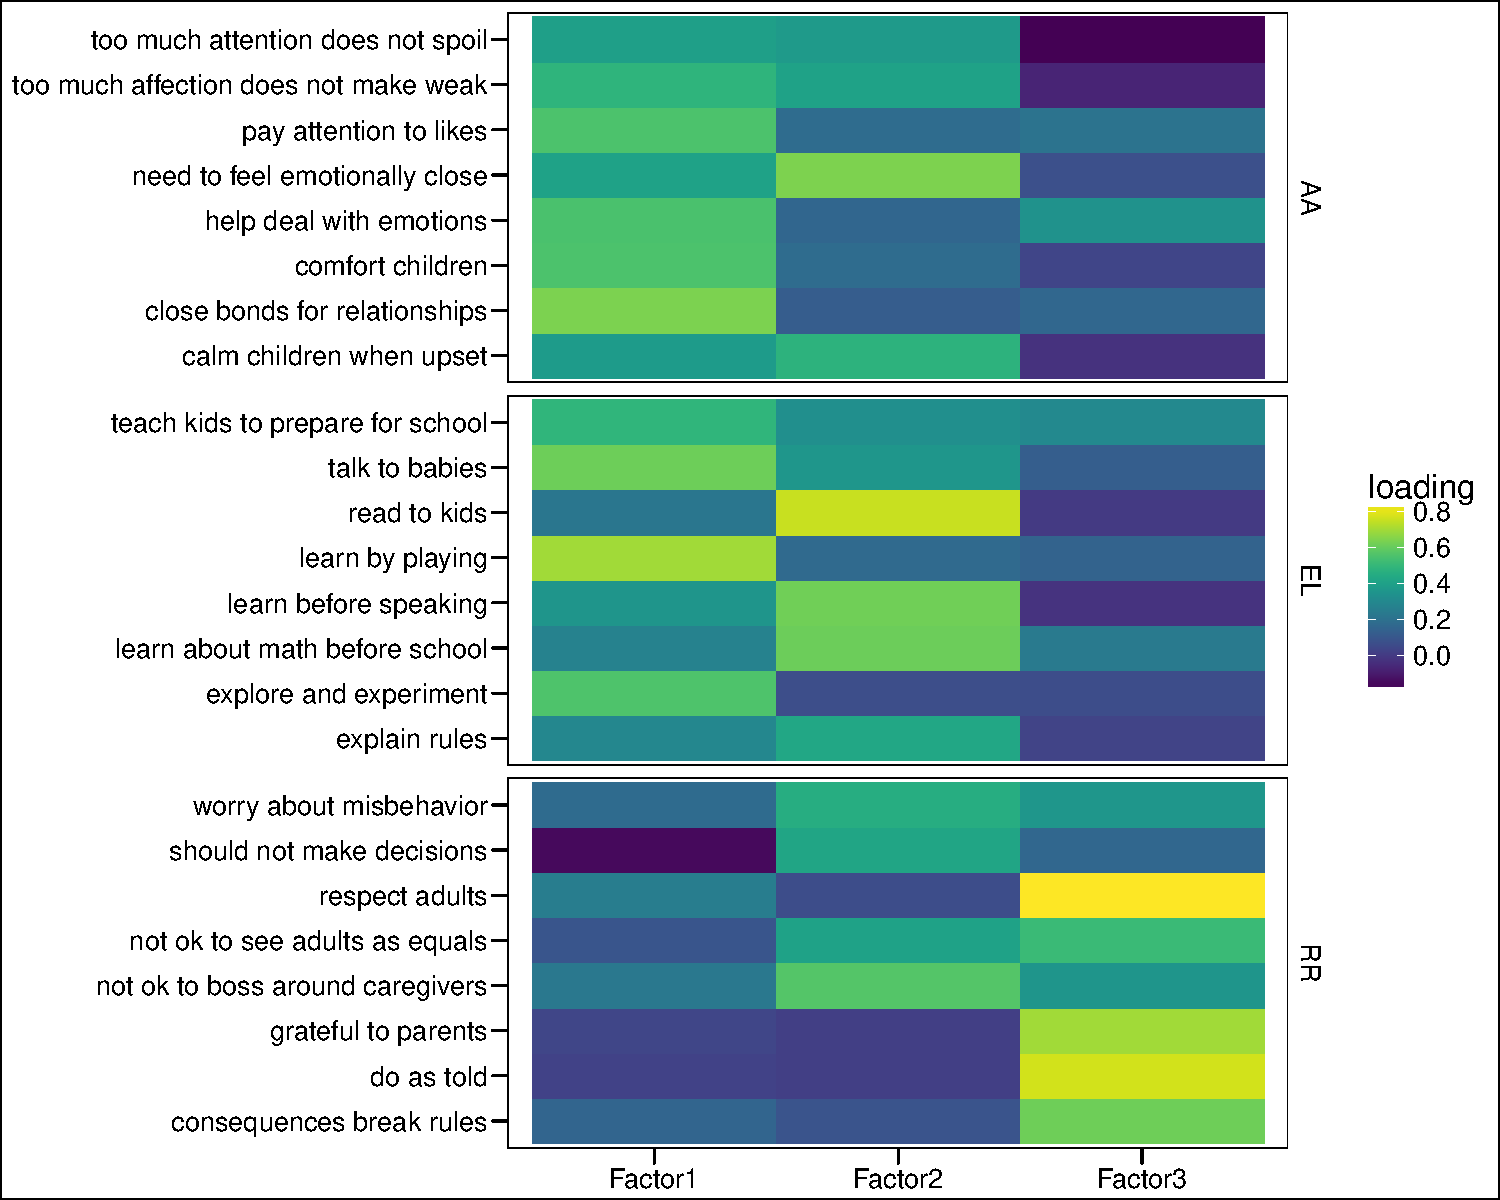
\includegraphics{PAQ_paper_files/figure-latex/factors-1.pdf}
\caption{\label{fig:factors}Factor loadings on individual PAQ questions.}
\end{figure}

\subsection{Item generation and dimension
reduction}\label{item-generation-and-dimension-reduction}

In an initial phase of scale construction, we generated 27 statements
that described various attitudes about parenting and child development
that we predicted parents might differ on. We selected these items based
on a literature review of previous parenting research, including
existing measures and theories such as the Knowledge of Infant
Development Inventory (KIDI, MacPhee, 2002), Baumrind's parenting
framework, and theories of attachment parenting (Jones, Cassidy, \&
Shaver, 2014). Critically, although the present scale is theoretically
related to existing frameworks, the present scale differs from them in
that parents are asked about their attitudes, rather than their
knowledge or behaviors. Items included in the initial set related to
parents' emotional and physical relationships with their children, their
beliefs about children's early learning, beliefs about children's
autonomy, and other topics.

We administered the initial scale to 250 adults on Amazon's Mechanical
Turk (Mturk). Participants used a 7-point Likert scale to report the
degree to which they agreed with each statement from 0 (Do not Agree) to
6 (Strongly Agree). We began by conducting exploratory factor analysis
(EFA) to assess the dimensionality of the scale. Based on the output of
a parallel analysis (Horn, 1965), we retained 5 factors in this initial
model. We subsequently dropped any items that had factor loadings less
than .40 on the relevant factor, as well as any items that had factor
loadings greater than .40 on another factor.

We repeated this process a total of 8 times. After several iterations,
the parallel analysis began returning 3 factors, so we retained 3
factors in subsequent factor analyses. The first factor appeared to
corresponded to a theory about affection and attachment and captured the
idea that emotionally close parent-child relationships are important for
development. The second factor corresponded to ideas around the
importance of fostering early learning. The third factor corresponded to
ideas around rules and respect, including children's autonomy and
behavioral control. We titled these factors Affection and Attachment
(AA), Early Learning (EL), and Rules and Respect (RR). Once we had
identified these categories, we dropped items belonging to each category
(based on factor loadings) if analyses revealed that Cronbach's alpha
for that category would be increased by dropping the item. We also added
new items that were theoretically consistent with the categories that
had emerged. Some items were rephrased such that half of the items in
each subscale were negatively worded to control for response sets (e.g.,
a tendency to rate all items highly, Simms, 2008).

\subsection{Final scale}\label{final-scale}

The final set of items comprising the three subscales is presented in
Table \ref{tab:items}. For the final sample, which consisted of 250
participants recruited on Mturk, Chronbach's alpha for the whole scale
was 0.90, for the AA subscale was 0.82, for the EL subscale was 0.83,
and for the RR subscale was 0.81. In sum, items within subscales are
highly correlated, but items across subscales are highly correlated as
well, which may reflect response biases to rate all items particularly
high or low.

We next examined the loadings of individual items onto the three factors
(Figure \ref{fig:loadings}). Items loaded onto the three factors roughly
consistent with our established subscales, although some items from the
AA subscale loaded onto both the AA and EL factors, and several items
from the EL subscale loaded more strongly onto the AA factor. Given the
partial overlap of the EL and AA factors, it is possible that
participants' responses on these items were driven to some extent by a
more general attitude towards more involved parenting.

\section{Survey Validation}\label{survey-validation}

\subsection{Study 1: Variability in parenting attitudes based on
demographic
factors}\label{study-1-variability-in-parenting-attitudes-based-on-demographic-factors}

\begin{figure}
\centering
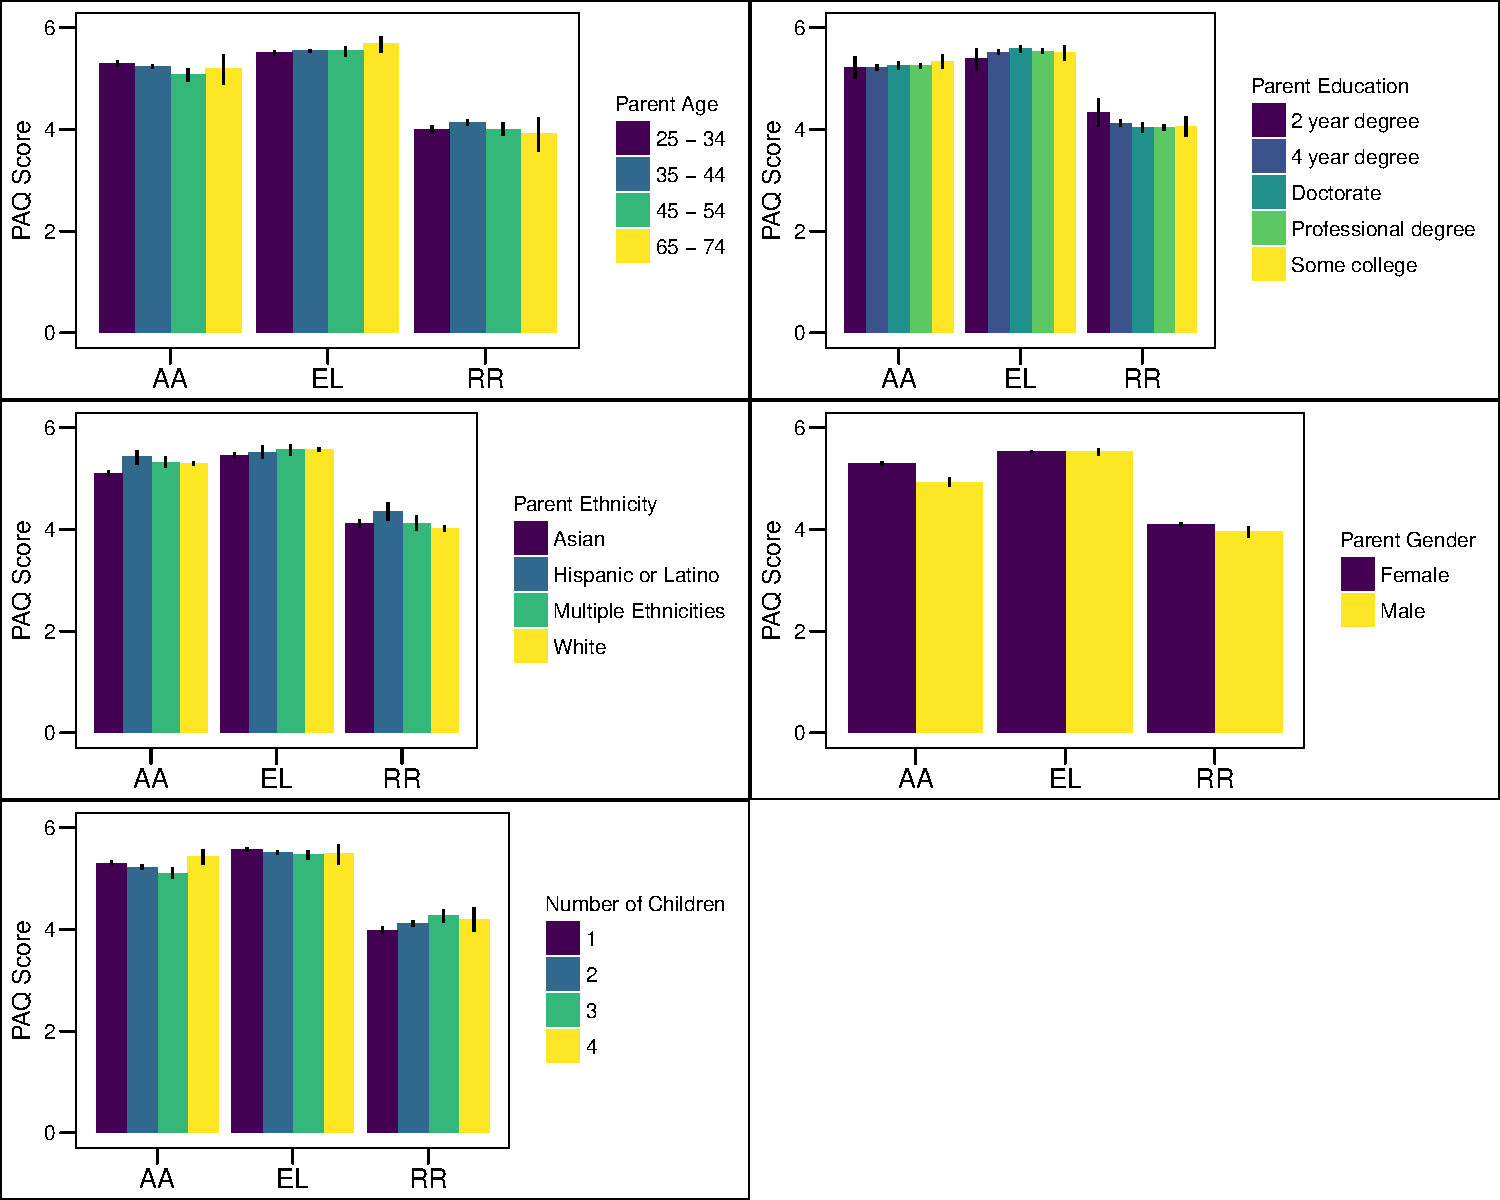
\includegraphics{PAQ_paper_files/figure-latex/demographics-1.pdf}
\caption{\label{fig:demographics}Demographic variability in PAQ scores.
Error bars represent +/-95\% CI computed by non-parametric bootstrap.}
\end{figure}

\begin{table}[H]
\centering
\caption{Results of separate bayesian ordinal logistic regressions of demographic factors on agreement with AA, EL, and RR attitudes.} 
\label{tab:demo}
\begin{tabular}{llrrrr}
  \hline
Subscale & Factor & Estimate & Est. Error & Lower 95\% CI & Upper 95\% CI \\ 
  \hline
AA & Parent Age & -0.00 & 0.01 & -0.01 & 0.01 \\ 
   & Hispanic or Latino & 0.72 & 0.20 & 0.34 & 1.11 \\ 
   & Multiple Ethnicities & 0.50 & 0.16 & 0.18 & 0.82 \\ 
   & White & 0.31 & 0.09 & 0.12 & 0.49 \\ 
   & Parent Education & 0.02 & 0.02 & -0.01 & 0.05 \\ 
   & Number of children & -0.14 & 0.05 & -0.24 & -0.03 \\ 
   & Male & -0.70 & 0.11 & -0.92 & -0.48 \\ 
   \hline
EL & Parent Age & 0.01 & 0.01 & -0.00 & 0.02 \\ 
   & Hispanic or Latino & 0.26 & 0.19 & -0.12 & 0.64 \\ 
   & Multiple Ethnicities & 0.56 & 0.17 & 0.22 & 0.90 \\ 
   & White & 0.44 & 0.09 & 0.25 & 0.62 \\ 
   & Parent Education & 0.02 & 0.02 & -0.01 & 0.05 \\ 
   & Number of children & -0.14 & 0.05 & -0.24 & -0.03 \\ 
   & Male & -0.18 & 0.11 & -0.41 & 0.04 \\ 
   \hline
RR & Parent Age & -0.00 & 0.01 & -0.01 & 0.01 \\ 
   & Hispanic or Latino & 0.27 & 0.20 & -0.11 & 0.67 \\ 
   & Multiple Ethnicities & -0.02 & 0.17 & -0.34 & 0.31 \\ 
   & White & -0.20 & 0.10 & -0.38 & -0.01 \\ 
   & Parent Education & -0.02 & 0.02 & -0.05 & 0.01 \\ 
   & Number of children & 0.15 & 0.06 & 0.04 & 0.25 \\ 
   & Male & -0.17 & 0.12 & -0.39 & 0.06 \\ 
   \hline
\end{tabular}
\end{table}

Approaches to parenting are known to differ across cultures and groups.
To better understand whether the parenting attitudes captured by our
survey reflect group differences, we examined average scores on the PAQ
subscales based on demographic factors. We administered the PAQ to 680
parents who were members of a local children's museum and subsequently
asked them to provide information about their gender, level of
education, age, ethnicity, and the number of children they have. Figure
\ref{fig:demographics} displays the average PAQ scores for each
demographic category.

To quantify any possible group differences, we fit separate Bayesian
mixed-effects ordinal regression models for each subscale (AA, EL, RR)
with the following structure, with likert ratings of agreement for each
item (1-6) entered as dependent measures:
\texttt{agreement\ rating\ \textasciitilde{}\ age\ +\ education\ +\ ethnicity\ +\ gender\ +\ number\ of\ children\ +\ (1\ \textbar{}\ subject)\ +\ (1\textbar{}\ item)}
Groups with fewer than 20 cases were removed from plots and analyses to
avoid overfitting. Although displayed as categorical for visual
simplicity in Figure \ref{fig:demographics}, parent age and education in
years were entered as continuous variables in the regression models.

Table \ref{tab:demo} displays the results of the regression analyses. We
found that stronger agreement with AA attitudes was associated with
identifying as Hispanic or Latino (\(\beta\) = 0.72, 95\% CI = 0.34 -
1.11), White (\(\beta\) = 0.31, 95\% CI = 0.12 - 0.49), or multiple
ethnicities (\(\beta\) = 0.50, 95\% CI = 0.18 - 0.82) compared to Asian
(the comparison level). Having a greater number of children was
associated with lower agreement with AA attitudes (\(\beta\) = -0.14,
95\% CI = -0.24 - -0.03), as was identifying as Male (\(\beta\) = -0.70,
95\% CI = -0.92 - -0.48). Parent education was not meaningfully
associated with AA scores.

We found that stronger agreement with EL scores was associated with
identifying as White (\(\beta\) = 0.44, 95\% CI = 0.25 - 0.62) or
multiple ethnicities (\(\beta\) = 0.56, 95\% CI = 0.22 - 0.90), and
having more children was associated with slightly lower agreement with
EL scores (\(\beta\) = -0.14, 95\% CI = -0.24 - -0.03). No other
demographic variables were related to EL scores.

Finally, we found that stronger agreement with RR attitudes was
associated with having a greater number of children (\(\beta\) = 0.15,
95\% CI = 0.04 - 0.25), and identifying as White was associated with
lower agreement with RR attitudes (\(\beta\) = -0.20, 95\% CI = -0.38 -
-0.01).

\subsection{Study 2: Relation of attitudes to parenting
behaviors}\label{study-2-relation-of-attitudes-to-parenting-behaviors}

\begin{figure}
\centering
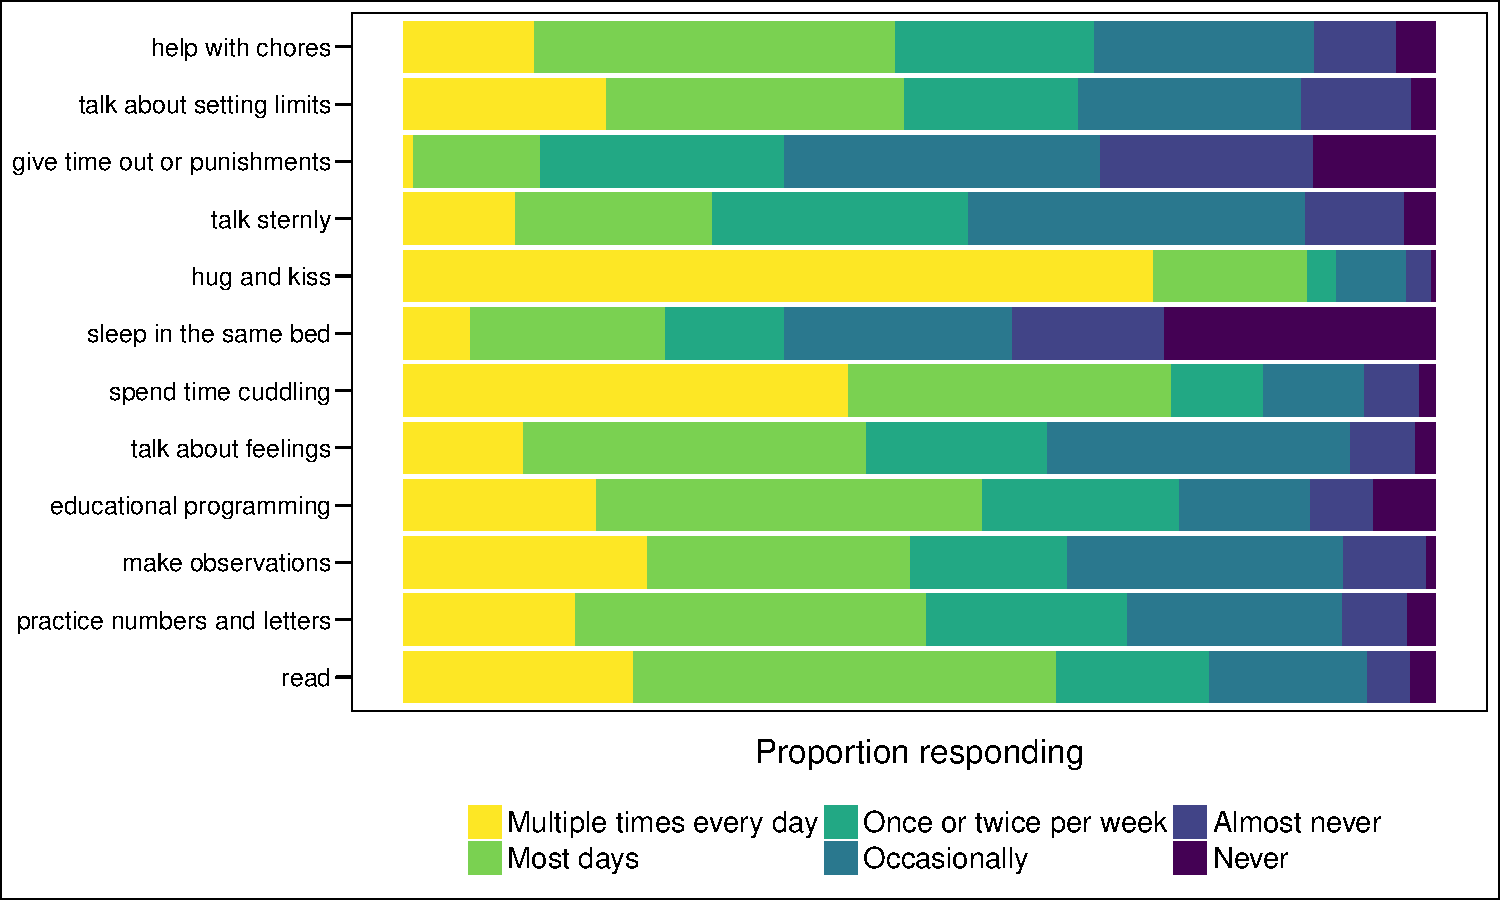
\includegraphics{PAQ_paper_files/figure-latex/behavefreq-1.pdf}
\caption{\label{fig:behavefreq}Frequencies of parenting activities reported
by parents.}
\end{figure}

\begin{figure}
\centering
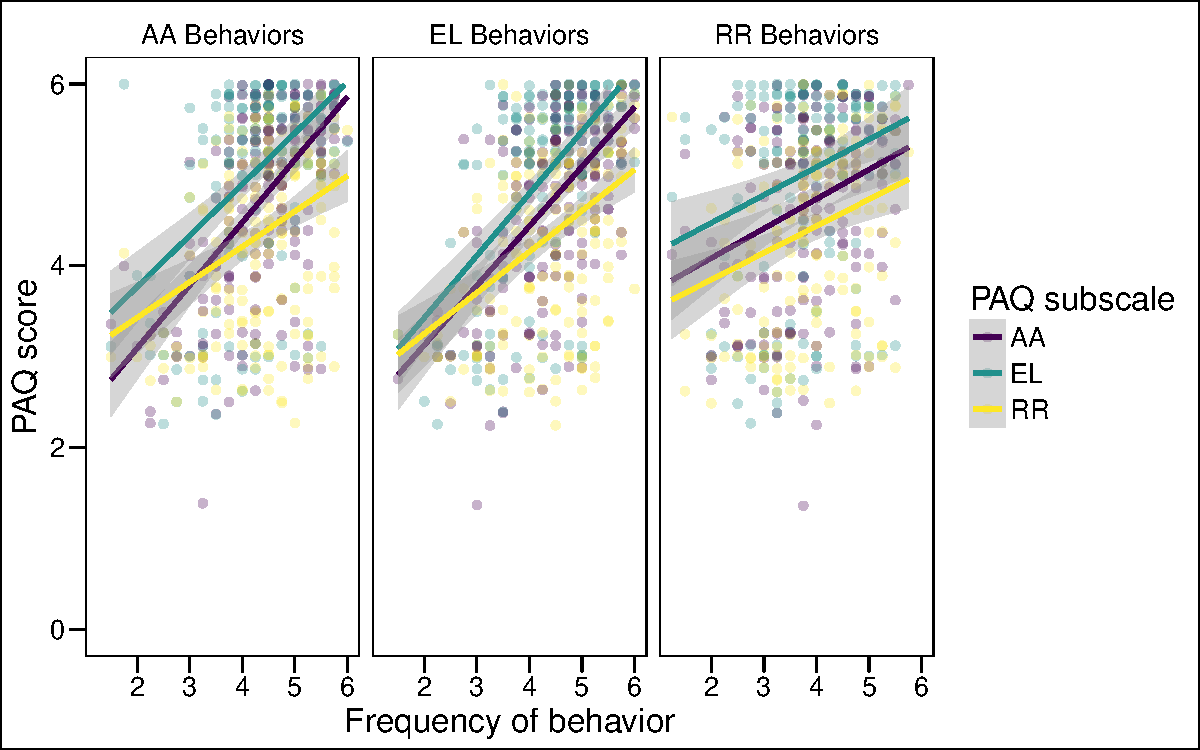
\includegraphics{PAQ_paper_files/figure-latex/behavepaq-1.pdf}
\caption{\label{fig:behavepaq}Relations between PAQ scores (Affection and
Attachment, Early Learning, and Rules and Respect) and the frequency of
parenting behaviors divided into the same categories.}
\end{figure}

\begin{table}[h]
\centering
\caption{Results of separate bayesian ordinal logistic regressions of PAQ scores and child age on frequency of parenting behaviors in Affection and Attachment (AA), Early Learning (EL), and Rules and Respect (RR) categories.} 
\label{tab:behavetab}
\begin{tabular}{llrrrr}
  \hline
Behavior Category & Factor & Estimate & Est. Error & Lower 95\% CI & Upper 95\% CI \\ 
  \hline
AA & AA PAQ score & 0.81 & 0.15 & 0.53 & 1.12 \\ 
   & RR PAQ score & -0.02 & 0.11 & -0.24 & 0.19 \\ 
   & EL PAQ score & -0.01 & 0.14 & -0.30 & 0.26 \\ 
   & Child Age & 0.01 & 0.01 & -0.00 & 0.02 \\ 
   \hline
EL & AA PAQ score & 0.37 & 0.18 & 0.02 & 0.71 \\ 
   & RR PAQ score & 0.20 & 0.13 & -0.06 & 0.45 \\ 
   & EL PAQ score & 0.52 & 0.18 & 0.18 & 0.88 \\ 
   & Child Age & 0.01 & 0.01 & -0.00 & 0.03 \\ 
   \hline
RR & AA PAQ score & 0.10 & 0.21 & -0.30 & 0.50 \\ 
   & RR PAQ score & 0.34 & 0.15 & 0.05 & 0.63 \\ 
   & EL PAQ score & 0.02 & 0.21 & -0.40 & 0.42 \\ 
   & Child Age & 0.03 & 0.01 & 0.01 & 0.05 \\ 
   \hline
\end{tabular}
\end{table}

\begin{table}[!h]

\caption{\label{tab:behavesents}Frequencies of parenting activities reported by parents.}
\centering
\fontsize{9}{11}\selectfont
\begin{tabular}[t]{>{\bfseries}l>{\raggedright\arraybackslash}p{40em}}
\toprule
Category & In the last month, how often did...\\
\midrule
AA & you and your child talk about feelings (e.g., when he/she was sad/angry)?\\
 & you and your child spend time cuddling?\\
 & your child sleep in the same bed as you?\\
 & you hug or kiss your child?\\
EL & you read to your child?\\
\addlinespace
 & you practice numbers or letters with your child?\\
 & you share facts or observations about the world when you were doing other tasks (e.g., did you know butter comes from cows? while shopping at the grocery store)?\\
 & your child watch educational programming (e.g., shows like Sesame Street) or play with educational apps (e.g., apps designed to teach numbers, colors, shapes, etc.) on a tablet or mobile device?\\
RR & you talk sternly to your child when he/she did something you dont want?\\
 & you give your child time out or other punishments for acting out?\\
\addlinespace
 & you talk about setting limits with your child (e.g., only 10 minutes of screen time or no hitting)?\\
 & your child help or try to help with chores or tasks (including cleaning up his/her toys)?\\
\bottomrule
\end{tabular}
\end{table}

Another way of assessing the ecological validity of the PAQ is to ask
whether the parenting attitudes it measures are related to actual
parenting behaviors. For example, do parents who strongly agree with
items on the Early Learning subscale read to their children more often?
Do parents who strongly endorse items on the Rules and Respect subscale
give more time-outs? To assess this, we asked a sample of 250 parents on
Mturk to complete the PAQ and then rate the frequency with which they
engaged in a number of parenting behaviors, focusing on the prior month
(Table \ref{tab:behavesents}). We elicited responses about 12 different
behaviors, with four corresponding to each PAQ category. Parents chose
between the following frequency options: \enquote{Multiple times per
day}, \enquote{Most days}, \enquote{Once or twice per week,}
\enquote{Occasionally,} \enquote{Almost never,} \enquote{Never,} and
\enquote{My child is too young for this.} Parents who did not have
children under the age of 5 were excluded from analyses, as were any
responses of \enquote{My child is too young for this.}

The distribution of frequencies that parents reported is displayed in
Figure \ref{fig:behavefreq}. To assess whether parenting behaviors are
associated with parenting attitudes, we calculated participants' average
PAQ subscale scores and fit separate bayesian ordinal logistic
mixed-effects regressions for the three cateogories of behaviors with
the following structure:
\texttt{behavior\ frequency\ \textasciitilde{}\ AA\ PAQ\ score\ +\ EL\ PAQ\ score\ +\ RR\ PAQ\ score\ +\ child\ age\ +\ (1\ \textbar{}\ subject)\ +\ (1\textbar{}\ item)}
(Table \ref{tab:behavetab}). The relation between PAQ scores and
behavior frequencies are presented in Figure \ref{fig:behavepaq}.

We found that the frequency of AA behaviors was positively associated
with AA attitudes (\(\beta\) = 0.81, 95\% CI = 0.53 - 1.12), but not RR
or EL attitudes or child age. Frequency of EL behaviors was positively
associated with stronger agreement with both AA (\(\beta\) = 0.37, 95\%
CI = 0.02 - 0.71) and EL attitudes (\(\beta\) = 0.52, 95\% CI = 0.18 -
0.88). The frequency of RR behaviors was positively associated with
stronger RR attitudes (\(\beta\) = 0.34, 95\% CI = 0.05 - 0.63), and to
a lesser extent, child age (\(\beta\) = 0.03, 95\% CI = 0.01 - 0.05).

These results suggest that parenting attitudes as assessed by the PAQ
have a meaningful relation to the actual behaviors parents engage in
with their children. This suggests that the current scale taps firmly
held beliefs that drive parents' decisions and behavior. It also
suggests that intervening on these beliefs may be an effective way of
promoting behavior change in parents, for example, to promote
opportunities for early learning. However, it is important to consider
that the present data are correlational and based on self-report. For
example, it is possible that participants' self-reported behaviors
capture their intentions rather than their actual behaviors, which would
likely be highly correlated with their self-reported attitudes. Future
work utilizing an intervention approach, and/or a diary method of
self-report, would help distinguish these possibilities.

\subsection{Study 3: Memory for new information about parenting and
child
development}\label{study-3-memory-for-new-information-about-parenting-and-child-development}

Parents' attitudes about parenting and child development may be an
important consideration for crafting interventions on parenting
behaviors or beliefs. There are frequent efforts to intervene on
parenting practices, for example, public service announcements telling
parents to read to their children; courses aimed at helping fathers
engage with their children; messages aimed at encouraging parents and
teachers to give children opportunities for free play. There is evidence
that existing lay theories can interact in surprising ways with this
type of messaging in other domains. Here we asked whether parents'
attitudes about parenting and child development would predict how they
uptake new information about child development versus an unrelated
topic.

\begin{figure}
\centering
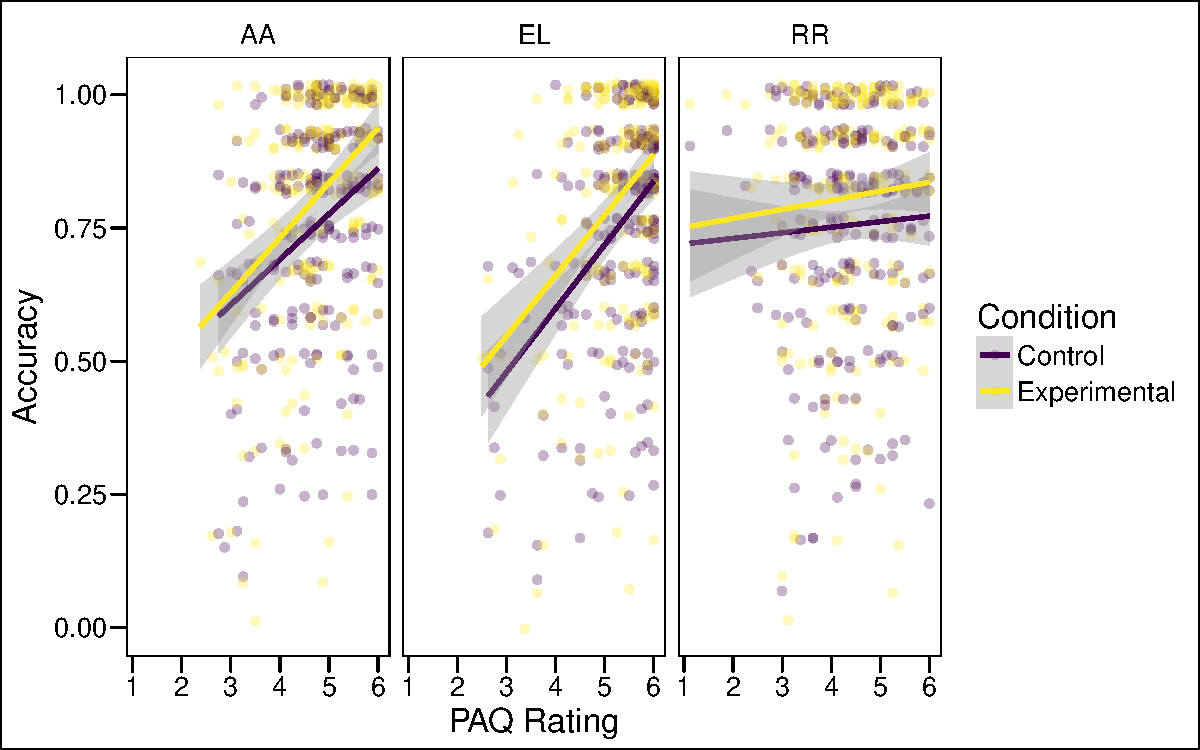
\includegraphics{PAQ_paper_files/figure-latex/uptake-1.pdf}
\caption{\label{fig:uptake}Relations between PAQ scores (Affection and
Attachment, Early Learning, and Rules and Respect) and the uptake of
information in experimental (child development-related) and control
articles.}
\end{figure}

\begin{table}[h]
\centering
\caption{Results of a bayesian logistic regression of PAQ scores and article topic (EL vs. control) on memory for information in articles.} 
\label{tab:uptake}
\begin{tabular}{lrrrr}
  \hline
Factor & Estimate & Est. Error & Lower 95\% CI & Upper 95\% CI \\ 
  \hline
EL Articles & -0.21 & 0.75 & -1.68 & 1.29 \\ 
  AA PAQ score & 0.05 & 0.15 & -0.25 & 0.35 \\ 
  RR PAQ score & -0.21 & 0.11 & -0.42 & 0.01 \\ 
  EL PAQ score & 0.82 & 0.16 & 0.52 & 1.14 \\ 
  AA PAQ score * EL Articles & 0.42 & 0.16 & 0.11 & 0.73 \\ 
  RR PAQ score * EL Articles & 0.02 & 0.11 & -0.19 & 0.23 \\ 
  EL PAQ score * EL Articles & -0.27 & 0.16 & -0.58 & 0.05 \\ 
   \hline
\end{tabular}
\end{table}

We asked 250 adults on Mturk to fill out the PAQ and then read four
popular press articles, two of which related to child development
({\textbf{???}}) and two of which related to other science topics
({\textbf{???}}). The articles were edited for length, and the order in
which the articles were presented was randomized. Next, participants
answered six four-alternative forced-choice questions testing their
memory and understanding of each article (24 total questions). We were
specifically interested in whether participants who agreed more strongly
with EL attitudes would better understand and remember the information
in the child development articles, which we predicted may have been
consistent with their existing views of development. Participants'
accuracy in relation to their average AA, EL and RR scores is displayed
in Figure \ref{fig:uptake}.

The average accuracy for control questions was 0.76(CI = 0.73 - 0.78)
and the average accuracy for experimenter questions was 0.81(CI = 0.73 -
0.83). There was no significant difference in accuracy between
conditions, t = -4.83, p = 0.00.

To assess whether participants who more strongly agreed with EL
attitudes were at an advantage for understanding and remembering the
child development articles they read, we fit a bayesian logistic
mixed-effects regression with the following structure:
\texttt{accuracy\ \textasciitilde{}\ AA\ PAQ\ score\ *\ article\ type\ +\ EL\ PAQ\ score\ *\ article\ type\ +\ RR\ PAQ\ score\ *\ article\ type\ +\ (article\ type\ \textbar{}\ subject)\ +\ (1\textbar{}\ item)}.
We excluded 7.70\% of responses from analyses because participants spent
fewer than 15 seconds reading the article, our pre-determined minimum
reading time.

We found that participants who agreed more strongly with EL attitudes
were more likely to answer memory questions correctly overall (\(\beta\)
= 0.82, 95\% CI = 0.52 - 1.14), but there was no interaction between EL
scores and article type, meaning that there was no advantage for people
with higher EL scores for understanding child development content in
particular. However, unexpectedly, there was an interaction between AA
attitudes and article type (\(\beta\) = 0.42, 95\% CI = 0.11 - 0.73),
such that people with stronger AA attitudes performed better on
questions about child development articles compared to control articles.
Rules and Respect attitudes did not predict memory for the articles.

In sum, our results suggest that people who believe more strongly in the
importance of early learning (i.e., those with higher EL PAQ scores) are
more likely to understand and recall details from science articles, but
they do not have a specific advantage for science articles related to
cognitive development during infancy. Contrary to our predictions, we
did find that people with higher AA scores had a specific advantage for
remembering the EL articles compared to control articles. Although the
present data cannot speak to why this might be, one possibility is that
people with higher AA scores have a stronger orientation towards content
about early childhood (compared to the unrelated content in the control
article) in general. These results could also reflect the fact that EL
and AA attitudes may overlap somewhat, as suggested by their respective
factor loadings, at least in the population we sampled for these
analyses.

\section{Discussion}\label{discussion}

In the present work, we established a new scale to measure people's
attitudes about parenting and child development in three categories:
Rules and Respect, Affection and Attachment, and Early Learning. These
subscales are meant to capture meaningful differences in how people view
child development and the relative importance of different parenting
behaviors. We subjected our new scale to psychometric evaluation, and
found acceptably high correlations among subscale items, as well as the
predicted factor structure across subscales. In addition, we found
meaningful differences in attitudes across demographic groups and we
observed the expected relations between parenting attitudes and
behaviors. We also found that PAQ subscale scores predicted
understanding and memory for new information in science articles, though
not in the predicted patterns, as people with higher AA scores had an
advantage for remembering the content of EL articles, but not people
with higher EL scores.

In sum, this work provides initial evidence that meaningful differences
in adults' attitudes about child development and parenting can be
assessed by our new scale.

Although the present studies provide initial evidence for the
reliability and validity of our parenting measure among the population
we sampled, which was predominantly White and highly educated, further
evidence across a broader range of participants would provide additional
support for the scale. In addition, future work should target predictive
validity by determining whether subscale scores differentially predict
parents observable behaviors with their children, such as the quality of
conversations they engage their child in.

Implicit theories are a powerful driver of human behavior. Sometimes,
the interaction between interventions and their subjects' underlying
beliefs can produce powerful, non-linear results ({\textbf{???}}). Thus,
given both the variability in attitudes towards parenting across
cultures and the importance of improving parenting outcomes, it behooves
us to understand implicit theories of parenting. The current work takes
a first step in this direction.

\newpage

\section{References}\label{references}

\begingroup
\setlength{\parindent}{-0.5in} \setlength{\leftskip}{0.5in}

\hypertarget{refs}{}
\hypertarget{ref-bransford1972}{}
Bransford, J. D., \& Johnson, M. K. (1972). Contextual prerequisites for
understanding: Some investigations of comprehension and recall.
\emph{Journal of Verbal Learning and Verbal Behavior}, \emph{11}(6),
717--726.

\hypertarget{ref-clark1995}{}
Clark, L. A., \& Watson, D. (1995). Constructing validity: Basic issues
in objective scale development. \emph{Psychological Assessment},
\emph{7}(3), 309--319.

\hypertarget{ref-furr2011}{}
Furr, M. (2011). \emph{Scale Construction and Psychometrics for Social
and Personality Psychology}. SAGE Publications Ltd.

\hypertarget{ref-hoff2003}{}
Hoff, E. (2003). The Specificity of Environmental Influence:
Socioeconomic Status Affects Early Vocabulary Development Via Maternal
Speech. \emph{Child Development}, \emph{74}(5), 1368--1378.

\hypertarget{ref-horn1965}{}
Horn, J. L. (1965). A rationale and test for the number of factors in
factor analysis. \emph{Psychometrika}, \emph{30}(2), 179--185.

\hypertarget{ref-huttenlocher2002}{}
Huttenlocher, J., Vasilyeva, M., Cymerman, E., \& Levine, S. (2002).
Language input and child syntax. \emph{Cognitive Psychology},
\emph{45}(3), 337--374.

\hypertarget{ref-jones2014}{}
Jones, J. D., Cassidy, J., \& Shaver, P. R. (2014). Parents
Self-Reported Attachment Styles A Review of Links with Parenting
Behaviors, Emotions, and Cognitions. \emph{Personality and Social
Psychology Review}, \emph{19}(1), 1088868314541858--76.

\hypertarget{ref-levine2004}{}
LeVine, R. A. (2004). \emph{Challenging Expert Knowledge: Findings from
an African Study of Infant Care and Development.} Praeger
Publishers/Greenwood Publishing Group.

\hypertarget{ref-macphee2002}{}
MacPhee, D. (2002). \emph{Knowledge of infant development inventory:
Manual}. Colorado: Colorado State University.

\hypertarget{ref-richman1992}{}
Richman, A. L., Miller, P. M., \& LeVine, R. A. (1992). Cultural and
educational variations in maternal responsiveness. \emph{Developmental
Psychology}, \emph{28}(4), 614--621.

\hypertarget{ref-rowe2008}{}
Rowe, M. L. (2008). Child-directed speech: relation to socioeconomic
status, knowledge of child development and child vocabulary skill.
\emph{Journal of Child Language}, \emph{35}(01), 185--205.

\hypertarget{ref-simms2008}{}
Simms, L. J. (2008). Classical and Modern Methods of Psychological Scale
Construction. \emph{Social and Personality Psychology Compass},
\emph{2}(1), 414--433.

\endgroup






\end{document}
